\large{
کمی به عقب برگردیم. هدف ما این بود که محیط را مدل سازی کنیم و داده‌های آن را ذخیره سازی و بازیابی کنیم. حال خوب است که از خود بپرسیم داده چیست؟
}
\\
\large{
در قسمت تحلیل، میخواهیم بدانیم که چه داده‌هایی داریم. این کار موسوم است به اسم مدل سازی معنایی داده‌ها، و منظور از این مدل‌سازی،‌ پیدا کردن بالاترین سطح انتزاع است به طوری که دیگر نشود سیستم را انتزاعی‌تر از آن دید. و این مدل‌سازی برای کاربران محیط قابل فهم است.
}

\graphicspath{ {./files/} }


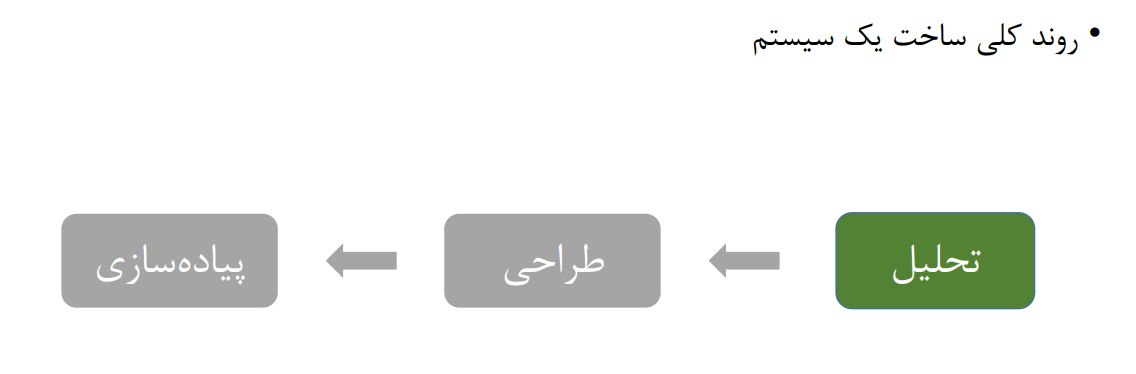
\includegraphics[scale=0.5]{2}


\large{
در اینجا لازم است بین داده و بین نوع داده تمایز قائل شویم. داده دقیقا یک اطلاعات است که از محیط دریافت میکنیم، مانند شماره دانشجویی یک دانشجوی خاص که در یک درس خاص ثبت نام کرده است. اما نوع داده، دانشجویان ثبت‌نامی در یک درس است.
}